\documentclass[conference]{IEEEtran}
\usepackage[utf8]{inputenc}
\usepackage[T1]{fontenc}
\usepackage{amsmath,amssymb}
\usepackage{graphicx}
\usepackage{booktabs}
\usepackage{hyperref}
\usepackage{cite}
\usepackage{xcolor}

\title{Trust Anchors for Agentic Scientific Computing:\\
Analytical Navier--Stokes Solutions as Verification Primitives\\in Multi-Agent AI Ecosystems}

\author{
\IEEEauthorblockN{Tatiana Petrova}
\IEEEauthorblockA{SEDAN -- SnT\\
University of Luxembourg\\
tatiana.petrova@uni.lu}
}

\begin{document}
\maketitle

%% ============================================================
%%  ABSTRACT
%% ============================================================
\begin{abstract}
The emergence of agentic AI systems---autonomous agents that discover, communicate, and collaborate through protocols such as MCP and A2A---is transforming scientific computing. In computational fluid dynamics, specialized AI agents (PINN solvers, neural operator surrogates, data assimilation modules) can now autonomously generate, exchange, and consume numerical solutions to the Navier--Stokes equations. However, this autonomy creates a critical \emph{trust problem}: when agents produce conflicting predictions with no human in the loop, how is correctness established? We argue that exact and semi-analytical solutions of the Navier--Stokes equations serve as \emph{trust anchors}---computationally verifiable ground truths that enable agents to self-validate, diagnose failure modes, and establish mutual trust without human intervention. Unlike traditional benchmarks, trust anchors are embedded in the agent's operational loop: evaluated at runtime, selected adaptively based on the current task, and used to maintain a dynamic, time-decaying trust score. We propose a Verified Multi-Agent Solver (VMAS) architecture with a structured interaction protocol, a dynamic trust ledger, and a diagnostic protocol mapping six documented failure modes of physics-informed machine learning to selective analytical solutions. As a proof of concept, we train three architecturally distinct PINN solvers (vanilla, Fourier-feature, and causal) on four trust anchors and show that the observed error patterns exhibit the predicted failure mode signatures---with instructive deviations that highlight sensitivity to training budget and architecture. We further demonstrate trust-informed routing, where the Orchestrator selects solvers based on diagnostic trust scores, achieving lower mean error than any single fixed solver on a heterogeneous problem set. Finally, we illustrate the full framework through a multi-agent atmospheric turbulence scenario coupling Navier--Stokes-based turbulence modeling with optical wave propagation.
\end{abstract}

\begin{IEEEkeywords}
Agentic AI, Web of Agents, trust anchors, Navier--Stokes equations, physics-informed neural networks, neural operators, multi-agent systems, verification, scientific computing
\end{IEEEkeywords}

%% ============================================================
%%  1. INTRODUCTION
%% ============================================================
\section{Introduction}

Scientific computing is entering an agentic era. Autonomous AI systems---capable of formulating subproblems, selecting methods, executing simulations, and interpreting results---are operational in weather prediction~\cite{Lam2023,Bi2023}, materials discovery~\cite{MatAgent2024}, and autonomous experimentation~\cite{Boiko2023}. In computational fluid dynamics (CFD), physics-informed neural networks (PINNs)~\cite{Raissi2019} and neural operators~\cite{Li2021FNO,Lu2021} can solve the Navier--Stokes (N--S) equations orders of magnitude faster than classical solvers, creating the possibility of AI agents that autonomously generate flow predictions on demand.

Concurrently, the Web of Agents (WoA) vision---tracing back through Multi-Agent Systems and the Semantic Web to modern LLM-powered frameworks---is crystallizing into practical protocols. Petrova et al.~\cite{PetrovaWoA2025} provide a comprehensive evolutionary analysis showing how the ``locus of intelligence'' has shifted from external data structures to the agent's internal model, enabling autonomous discovery and collaboration. Google's Agent-to-Agent (A2A) protocol~\cite{A2A2025} and Anthropic's Model Context Protocol (MCP)~\cite{MCP2024} provide standardized interfaces for agent interoperability. These developments make multi-agent scientific workflows---where a solver agent generates a prediction, a surrogate agent provides a fast approximation, and an assimilation agent fuses both with observational data---technically feasible.

But feasibility does not imply trustworthiness. When an autonomous PINN agent reports a velocity field, or an FNO agent predicts turbulence statistics, \emph{how does the system verify correctness?} In the absence of a human expert examining each output, the multi-agent system needs an \emph{internal verification mechanism}. This is the trust problem, and it is the agentic analogue of the classical validation challenge in scientific computing~\cite{Oberkampf2010}.

We propose that exact and semi-analytical solutions of the Navier--Stokes equations serve as \textbf{trust anchors} for agentic scientific computing. By analogy with root certificates in public-key infrastructure, a trust anchor is a known-good reference from which trust in other entities can be derived. Analytical N--S solutions satisfy the governing equations exactly (or to known perturbation order), are free from discretization errors, and can be evaluated to arbitrary precision---making them ideal primitives for automated verification.

This paper makes four contributions:
\begin{enumerate}
    \item We introduce the concept of \emph{trust anchors}, distinguishing them from traditional benchmarks through three functional requirements specific to the agentic context: runtime monitoring, adaptive test selection, and inter-agent arbitration (Section~\ref{sec:trust}).
    \item We propose the \emph{Verified Multi-Agent Solver} (VMAS) architecture with a structured interaction protocol, dynamic trust ledger, and diagnostic protocol mapping six PIML failure modes to selective trust anchors (Section~\ref{sec:architecture}).
    \item We provide a proof-of-concept experimental validation by training three architecturally distinct PINNs on four trust anchors, showing that error patterns exhibit the predicted failure mode signatures, while identifying sensitivity to training budget as a confounding factor (Section~\ref{sec:experiments}).
    \item We illustrate the full framework through a multi-agent atmospheric turbulence scenario (Section~\ref{sec:casestudy}).
\end{enumerate}


%% ============================================================
%%  2. BACKGROUND
%% ============================================================
\section{Background and Related Work}
\label{sec:background}

\subsection{The Web of Agents}

The concept of autonomous software agents collaborating on the Web has a three-decade history. Petrova et al.~\cite{PetrovaWoA2025} trace this evolution through four generations: from static single-purpose agents under FIPA standards~\cite{FIPA2002}, through socially aware MAS platforms~\cite{JADE2007} and Semantic Web agents~\cite{BernersLee2001}, to the current generation of LLM-powered agents with protocols like MCP~\cite{MCP2024} and A2A~\cite{A2A2025}. A key finding is the identification of a paradigm shift in the ``locus of intelligence'': from semantics encoded in external data to semantics embedded in the agent's core model. This shift enables flexible agents but raises challenges in trust and verification---especially acute in scientific computing where correctness is paramount.

Recent work on agentic AI for science includes autonomous research agents~\cite{AIScientist2024}, LLM-driven autonomous experimentation~\cite{Boiko2023}, and multi-agent systems for materials design~\cite{MatAgent2024}. Comprehensive surveys of LLM-based agent frameworks~\cite{Ferrag2025,Wang2024agents} catalog architectures and protocols but do not address the verification problem systematically.

\subsection{Physics-Informed Machine Learning}

PINNs~\cite{Raissi2019} solve PDEs by training a neural network to minimize a composite loss:
\begin{equation}\label{eq:PINN-loss}
  \mathcal{L}(\theta) = \lambda_r\,\mathcal{L}_r + \lambda_b\,\mathcal{L}_b
    + \lambda_i\,\mathcal{L}_i + \lambda_d\,\mathcal{L}_d,
\end{equation}
where $\mathcal{L}_r$ penalizes the PDE residual, $\mathcal{L}_b$ and $\mathcal{L}_i$ enforce boundary and initial conditions, and $\mathcal{L}_d$ matches data. Specialized architectures such as NSFnets~\cite{Park2021} use divergence-free formulations. Neural operators---including the Fourier Neural Operator (FNO)~\cite{Li2021FNO}, DeepONet~\cite{Lu2021}, and Physics-Informed Neural Operators (PINO)~\cite{Li2023PINO}---learn mappings between function spaces with up to three orders of magnitude speedup. The unified framework of Kovachki et al.~\cite{Kovachki2023} encompasses graph neural operators and low-rank factorizations. AI-driven weather models such as FourCastNet~\cite{Pathak2022} demonstrate that these architectures scale to global atmospheric prediction.

Despite these advances, PIML methods exhibit well-documented failure modes: spectral bias~\cite{Rahaman2019}, gradient pathologies~\cite{Wang2021}, temporal error accumulation, and poor parametric generalization~\cite{Hao2024}. In a human-supervised workflow, these failures are caught by expert inspection. In an agentic workflow, they must be caught \emph{automatically}.

\subsection{Analytical Solutions of the Navier--Stokes Equations}

The incompressible N--S equations,
\begin{equation}\label{eq:NS}
  \frac{\partial \mathbf{v}}{\partial t} + (\mathbf{v}\cdot\nabla)\mathbf{v}
    = -\frac{1}{\rho}\nabla p + \nu\,\Delta\mathbf{v},
  \qquad \nabla\cdot\mathbf{v}=0,
\end{equation}
admit exact solutions for specific geometries~\cite{Drazin2006,Wang1991}: the Lamb--Oseen decaying vortex, the Burgers vortex with axial stretching~\cite{Burgers1948}, the Sullivan two-cell tornado vortex~\cite{Sullivan1959}, the Jeffery--Hamel converging channel flow~\cite{Jeffery1915}, the von K\'arm\'an swirling flow~\cite{Karman1921}, Falkner--Skan boundary layers~\cite{Schlichting2017}, and the Taylor--Green vortex~\cite{Brachet1983}. Generalized Beltrami flows~\cite{Burmasheva2023} and nonlinear PDE handbooks~\cite{Polyanin2004} further expand the catalog.

For the compressible N--S system, perturbation methods yield semi-analytical results. By expanding in powers of a small vorticity parameter, the nonlinear system reduces to a hierarchy of linear parabolic problems with constant coefficients, solvable via integral transforms and numerical quadrature on Korobov grids~\cite{PetrovaShugaev2015}. Such approaches have produced results for cylindrical vortex acoustics, oscillatory flow dynamics, and coupled fluid-optical problems---none of which have been adopted as PIML benchmarks despite providing discretization-free reference solutions.

The catalog of known N--S solutions encompasses hundreds of families~\cite{Drazin2006}, yet only a handful (Taylor--Green, Kovasznay, lid-driven cavity) are routinely used in PIML validation~\cite{Hao2024}. We argue that this untapped resource acquires new significance in the agentic context.


%% ============================================================
%%  3. FROM BENCHMARKS TO TRUST ANCHORS
%% ============================================================
\section{From Benchmarks to Trust Anchors}
\label{sec:trust}

\subsection{Why Benchmarks Are Not Enough for Agents}

A benchmark is a \emph{one-time, offline evaluation}: a researcher runs a solver on a test case, compares with the reference, publishes a table. The intelligence is in the human, not in the test. In an agentic system, this workflow breaks down in three specific ways:

\textbf{(i)~Continuous operation.} A Solver Agent runs indefinitely on a stream of heterogeneous problems. Its reliability may degrade over time (model drift, distribution shift, numerical instabilities). A benchmark provides a snapshot; what is needed is a \emph{runtime monitor} that periodically checks the agent during operation---analogous to a heartbeat signal in distributed systems.

\textbf{(ii)~Adaptive test selection.} A human picks benchmarks based on expertise. An autonomous system must decide \emph{which} tests to run for a \emph{given} problem. When a Solver receives a vortex problem with acoustic coupling, the verification system should prioritize multi-scale anchors over boundary layer tests. This requires reasoning about the \emph{diagnostic relevance} of each anchor to the current task.

\textbf{(iii)~Arbitration.} When two Solvers produce conflicting results, benchmarks cannot resolve the conflict. A trust system can: if Agent~A has passed vortex-acoustic anchors but Agent~B has not, the system has a principled basis for preferring Agent~A on vortex-acoustic problems. This requires maintaining and propagating \emph{trust state}---a dynamic quantity that static benchmarks do not generate.

We define a \textbf{trust anchor} as a reference solution that is \emph{embedded in the agent's operational loop}: evaluated at runtime, selected adaptively, and used to maintain dynamic trust state. The same Lamb--Oseen solution is a benchmark when a human evaluates a paper, and a trust anchor when a Validator Agent uses it to certify a Solver before forwarding its output. The distinction is functional, not mathematical.

\subsection{Trust Distance}

Beyond standard requirements (exactness, computability), trust anchors must support \emph{trust-distance computation}: for any novel problem~$P$, the system must estimate how far~$P$ lies from each anchor~$A_i$:
\begin{equation}\label{eq:trust-distance}
  d(P, A_i) = \sqrt{\sum_k w_k \left(\frac{\pi_k(P) - \pi_k(A_i)}{\Delta\pi_k}\right)^2},
\end{equation}
where $\pi_k$ are relevant physical parameters (Re, Mach, geometry ratio), $\Delta\pi_k$ are characteristic scales, and $w_k$ are weights. The Validator assigns higher confidence when $d(P, A_i)$ is small for anchors the Solver has passed.


%% ============================================================
%%  4. VMAS ARCHITECTURE
%% ============================================================
\section{Verified Multi-Agent Solver Architecture}
\label{sec:architecture}

\subsection{System Overview and Interaction Protocol}

The VMAS comprises four agent types:
\begin{itemize}
    \item \textbf{Solver Agents} ($\mathcal{S}_1,\ldots,\mathcal{S}_n$): each wraps a PIML method and exposes a \texttt{solve(problem)} interface via MCP~\cite{MCP2024}.
    \item \textbf{Validator Agent} ($\mathcal{V}$): maintains the trust anchor database and a \emph{trust ledger}---a persistent, time-stamped record of each Solver's performance.
    \item \textbf{Orchestrator Agent} ($\mathcal{O}$): receives user problems, computes trust distances, and routes to the Solver with the highest task-relevant trust score.
    \item \textbf{Data Agent} ($\mathcal{D}$): provides observational data for problems without analytical solutions.
\end{itemize}

In the A2A paradigm~\cite{A2A2025}, agents publish ``Agent Cards'' describing capabilities. We extend this with a \emph{trust profile}: the list of passed anchors, tolerance levels, and timestamps. This extends interoperability patterns described in recent surveys~\cite{Ferrag2025,Wang2024agents}. The interaction protocol is described in Fig.~\ref{fig:vmas}. We note that the protocol is presented as a structured design rather than a formal specification with proof obligations; formal verification of trust update properties (e.g., routing optimality guarantees) remains future work.

\begin{figure}[t]
\centering
\fbox{\parbox{0.92\columnwidth}{\small\ttfamily
\textbf{VMAS Interaction Protocol}\\[4pt]
1.~~User $\to$ $\mathcal{O}$: submit(problem P)\\
2.~~$\mathcal{O}$: compute $d(P, A_i)$ for all anchors\\
\hspace*{1.5em}identify relevant anchor set $\{A_{i^*}\}$\\
3.~~$\mathcal{O}$ $\to$ $\mathcal{V}$: get\_trust\_scores($\mathcal{S}_j$, $\{A_{i^*}\}$)\\
4.~~$\mathcal{V}$: lookup trust ledger\\
\hspace*{1.5em}\textbf{if} stale or missing:\\
\hspace*{2.5em}run\_anchors($\mathcal{S}_j$, $\{A_{i^*}\}$)\\
\hspace*{1.5em}return scores[$\mathcal{S}_j$][$A_{i^*}$]\\
5.~~$\mathcal{O}$: select $\mathcal{S}_{best}$ = argmax(scores)\\
6.~~$\mathcal{O}$ $\to$ $\mathcal{S}_{best}$: solve(P)\\
7.~~$\mathcal{S}_{best}$ $\to$ $\mathcal{O}$: solution U\\
8.~~$\mathcal{O}$ $\to$ $\mathcal{V}$: spot\_check(U, P)\\
9.~~$\mathcal{V}$: \textbf{if} $d(P, A_i) < \delta$ for some $A_i$:\\
\hspace*{2.5em}compare $\|U - U_{A_i}\|$ at shared params\\
\hspace*{2.5em}update trust ledger\\
\hspace*{1.5em}return \{verified, diagnostics: F1..F6\}\\
10. $\mathcal{O}$ $\to$ User: solution + trust\_report
}}
\caption{VMAS interaction protocol. Steps 2--5: trust-informed routing. Steps 8--9: runtime spot-checking.}
\label{fig:vmas}
\end{figure}

\subsection{What Makes the Validator an Agent, Not a Test Script}

A static test suite runs fixed tests in fixed order and returns pass/fail. The Validator differs in three capabilities:

\textbf{(a)~Adaptive anchor selection.} Given problem~$P$, the Validator computes $d(P, A_i)$ and selects the most diagnostically relevant subset. Vortex-dominated problems trigger vortex anchors; boundary-layer problems trigger Falkner--Skan.

\textbf{(b)~Dynamic trust ledger.} Each Solver's trust is a continuous, time-decaying quantity:
\begin{equation}\label{eq:trust-score}
  T(\mathcal{S}_j, t) = \sum_i w_i\, \tau(\mathcal{S}_j, A_i, t_i)\, e^{-\lambda(t - t_i)},
\end{equation}
where $\tau = 1$ if the Solver passed anchor $A_i$ at time $t_i$ within tolerance $\epsilon_i$, and $\lambda$ controls trust decay. A Solver certified a month ago has lower trust than one certified an hour ago.

\textbf{(c)~Diagnostic reasoning.} On failure, the Validator returns a structured message \texttt{\{agent, failed\_anchor, failure\_mode, recommendation\}} to the Orchestrator, enabling intelligent rerouting.

\subsection{Trust Anchor Suite and Diagnostic Map}

Table~\ref{tab:anchors} maps trust anchors to the six failure modes documented in the PIML literature: spectral bias (F1,~\cite{Rahaman2019}), temporal drift (F2,~\cite{Wang2021}), parametric overfitting (F3,~\cite{Li2021FNO}), multi-scale decoupling (F4), boundary artifacts (F5,~\cite{Hao2024}), and conservation violation (F6,~\cite{Park2021}).

\begin{table}[t]
\centering
\caption{Trust anchor suite. $\bullet$~primary diagnostic; $\circ$~secondary.}
\label{tab:anchors}
\small
\begin{tabular}{@{}lcccccc@{}}
\toprule
\textbf{Trust Anchor} & \textbf{F1} & \textbf{F2} & \textbf{F3} & \textbf{F4} & \textbf{F5} & \textbf{F6} \\
\midrule
Lamb--Oseen vortex         &      & $\bullet$ &      &      &      & $\circ$ \\
Stokes oscil.\ plate       & $\bullet$ & $\circ$ &      &      &      &      \\
Burgers vortex              &      &      &      &      &      & $\bullet$ \\
Sullivan vortex             &      &      &      &      & $\bullet$ &      \\
Jeffery--Hamel flow         &      &      & $\bullet$ &      &      &      \\
Falkner--Skan family        &      &      & $\bullet$ &      & $\circ$ &      \\
Cyl.\ vortex acoustics     & $\circ$ &      & $\bullet$ & $\bullet$ &      &      \\
Vortex flow oscillations    & $\bullet$ & $\bullet$ &      & $\circ$ &      &      \\
N--S turb.\ atmosphere      & $\circ$ & $\circ$ &      & $\bullet$ &      & $\circ$ \\
\bottomrule
\end{tabular}
\end{table}

The assignments follow from the mathematical structure of each solution. For example, the Lamb--Oseen vortex has no oscillatory content and no parameter dependence---isolating pure temporal accuracy (F2). The Stokes plate contains a single frequency $\omega$---directly probing spectral resolution (F1). The cylindrical vortex acoustics problem~\cite{PetrovaShugaev2015} couples slow vortex dynamics ($\tau_{\mathrm{vortex}} \sim R_0/(\varepsilon c_0)$) with fast acoustic radiation ($\tau_{\mathrm{ac}} \sim R_0/c_0$), with ratio $\sim 1/\varepsilon \gg 1$---probing multi-scale decoupling (F4). The vortex flow oscillations~\cite{PetrovaShugaev2012} involve a superposition of multiple analytically determined frequencies with different decay rates governed by the transport coefficients---probing F1+F2 jointly.

\subsection{Three-Stage Diagnostic Protocol}
\label{sec:diag}

\textbf{Stage~1: Certification.} Before admission, a Solver must pass baseline anchors: Lamb--Oseen (F2), Stokes plate (F1), Poiseuille flow (F5). Certification is time-stamped and decays per Eq.~\eqref{eq:trust-score}.

\textbf{Stage~2: Diagnosis.} On suspicious output, the Validator selects anchors based on trust distance to the current problem. If the Solver passes Lamb--Oseen but fails vortex oscillations~\cite{PetrovaShugaev2012}, the diagnosis is F1 (spectral bias)---the Solver captures the dominant mode but misses overtones.

\textbf{Stage~3: Stress testing.} For high-stakes problems: cylindrical vortex acoustics~\cite{PetrovaShugaev2015} (F3+F4), vortex oscillations~\cite{PetrovaShugaev2012} (F1+F2), and N--S atmospheric turbulence (F4 multi-physics; Section~\ref{sec:casestudy}).

\subsection{Trust Propagation and Limitations}

Trust anchors provide necessary but not sufficient conditions for correctness. Most anchors correspond to laminar, low-to-moderate Re flows, while PIML is most needed for high-Re turbulence. The trust distance~\eqref{eq:trust-distance} quantifies this gap: large $d(P, A_i)$ should trigger ensemble methods or human oversight. The suite is most effective as a \emph{filter for known failure modes}, not a guarantee of correctness in novel regimes.


%% ============================================================
%%  5. EXPERIMENTS
%% ============================================================
\section{Experimental Validation}
\label{sec:experiments}

\subsection{Setup}

\textbf{Trust anchors.} We implement four anchors as closed-form functions:

\emph{A1: Lamb--Oseen vortex} (targets F2):
$v_\theta(r,t) = \frac{\Gamma_0}{2\pi r}[1 - e^{-r^2/4\nu t}].$
Evaluated over $t \in [t_0, 50\,t_0]$, $t_0 = R_0^2/\nu$.

\emph{A2: Stokes oscillating plate} (targets F1):
$u(z,t) = U_0\, e^{-z\sqrt{\omega/2\nu}} \cos(\omega t - z\sqrt{\omega/2\nu}).$
Evaluated at $\omega \in \{\omega_1, 2\omega_1, 4\omega_1, 8\omega_1\}$.

\emph{A3: Burgers vortex} (targets F6):
$v_\theta(r) = \frac{\Gamma_0}{2\pi r}[1 - e^{-\alpha r^2/2\nu}]$, $v_r = -\frac{\alpha}{2}r$, $v_z = \alpha z.$
Steady-state; we measure circulation error $|\oint \hat{v}_\theta\,r\,d\theta - \Gamma_0|/\Gamma_0$.

\emph{A4: Kovasznay flow} (baseline): standard 2D steady solution at $\mathrm{Re}=20$~\cite{Drazin2006}.

\textbf{Solvers.} Three PINN variants via DeepXDE, same training budget (2k iterations, Adam, $\mathrm{lr}=10^{-3}$, 3k interior + 500 boundary collocation points, 3 seeds per experiment):
\begin{itemize}
  \item \textbf{S1: Vanilla PINN} (4 layers $\times$ 64, $\tanh$). Predicted: weak on F1, F2.
  \item \textbf{S2: Fourier-Feature PINN}~\cite{Wang2021} (256-dim random Fourier input features, $\sigma = 10$). Predicted: improved F1, weak F2.
  \item \textbf{S3: Causal PINN} (two-phase training: warm-up followed by low-LR refinement). Predicted: improved F2, weak F1.
\end{itemize}
\textbf{Note on training budget.} The training budget was intentionally kept modest to enable a complete 72-run experiment on CPU hardware. This means absolute error values are higher than state-of-the-art for well-tuned PINNs, and the Fourier-Feature architecture (S2), which maps inputs to a 256-dimensional feature space, is systematically disadvantaged on low-iteration budgets. The diagnostic value lies not in the absolute error magnitudes but in the \emph{relative patterns across solvers and anchors}: which solver--anchor pairs produce the largest and smallest errors, and whether these patterns match the predicted failure mode signatures.

\textbf{Metrics.} Global relative $L^2$ error $\epsilon_{L^2} = \|\hat{\mathbf{u}} - \mathbf{u}_{\mathrm{exact}}\|_{L^2}/\|\mathbf{u}_{\mathrm{exact}}\|_{L^2}$, plus anchor-specific diagnostics: temporal error profile $\epsilon(t)$ for A1, frequency response $\epsilon(\omega)$ for A2, circulation error $\delta\Gamma(r)$ for A3.


\subsection{Diagnostic Pattern Validation}

Table~\ref{tab:results} presents global errors for all Solver--Anchor pairs.

\begin{table}[t]
\centering
\caption{Global relative $L^2$ errors (\%) for three PINNs on four trust anchors.}
\label{tab:results}
\small
\begin{tabular}{@{}lcccc@{}}
\toprule
 & A1 (Lamb-Oseen) & A2 (Stokes) & A3 (Burgers) & A4 (Kovasznay) \\
 & F2: drift & F1: spectral & F6: conserv. & baseline \\
\midrule
S1 (Vanilla)  & $45.28 \pm 36.54$ & $2.77 \pm 0.20$ & $24.55 \pm 0.55$ & $207.35 \pm 8.70$ \\
S2 (Fourier)  & $486.92 \pm 55.92$ & $73.75 \pm 7.06$ & $9.04 \pm 3.94$ & $41.38 \pm 3.69$ \\
S3 (Causal)  & $20.17 \pm 3.54$ & $3.22 \pm 0.22$ & $24.55 \pm 0.55$ & $194.18 \pm 7.58$ \\
\bottomrule
\end{tabular}
\end{table}

\textbf{Predicted pattern.} If diagnostic assignments are correct: (i)~S1 shows highest error on A1 and A2 at high $\omega$; (ii)~S2 improves on A2 but not A1; (iii)~S3 improves on A1 but not A2; (iv)~all comparable on A3 and A4.

The predicted diagnostic pattern is partially confirmed, with instructive deviations. On the Lamb--Oseen anchor (A1, targeting~F2), S3~(Causal) achieves $20.17 \pm 3.54\%$ versus S1's $45.28 \pm 36.54\%$---a $55\%$ improvement in mean error with dramatically reduced variance, confirming that causal temporal weighting mitigates drift. S2~(Fourier), however, fails on A1 ($486.92\%$), revealing that its high-dimensional Fourier feature mapping ($256$-dim input) requires substantially more training iterations, an observation consistent with the known computational cost of random Fourier features~\cite{Rahaman2019}.

On the Stokes plate (A2, targeting~F1), S1~(Vanilla) and S3~(Causal) both achieve low errors ($2.77\%$ and $3.22\%$, respectively), while S2 shows $73.75\%$. This \emph{apparent} reversal---S2 worse, not better, on the spectral anchor---reflects a confound between convergence cost and spectral capability. The A2 entry in Table~\ref{tab:results} is evaluated at the \emph{base frequency} $\omega_1$, where the problem is easy for a standard MLP but the 256-dim Fourier mapping has not converged within the training budget. The true spectral diagnosis requires the multi-frequency protocol of Section~5.3, where S2's advantage at high $\omega$ becomes decisive (Fig.~\ref{fig:spectral}). On the Burgers vortex (A3, targeting~F6), S2 achieves the lowest error ($9.04\%$), while S1 and S3 are comparable ($24.55\%$), suggesting that Fourier features improve steady-state accuracy. On the Kovasznay baseline (A4), S2 again outperforms ($41.38\%$ vs.\ $>190\%$ for S1 and S3), revealing that the vanilla and causal architectures struggle with the 2D steady N--S system at the given training budget.

The key finding is \emph{diagnostic selectivity}: the Lamb--Oseen anchor cleanly separates S3 (designed for temporal accuracy) from S1 and S2, while the Burgers and Kovasznay anchors reveal that Fourier features aid spatial representation at the cost of slower convergence on temporal problems. This validates the core claim that trust anchors can diagnose specific PIML failure modes and that different anchors expose different architectural strengths.

\subsection{Spectral Bias Diagnosis}

\begin{figure}[t]
\centering
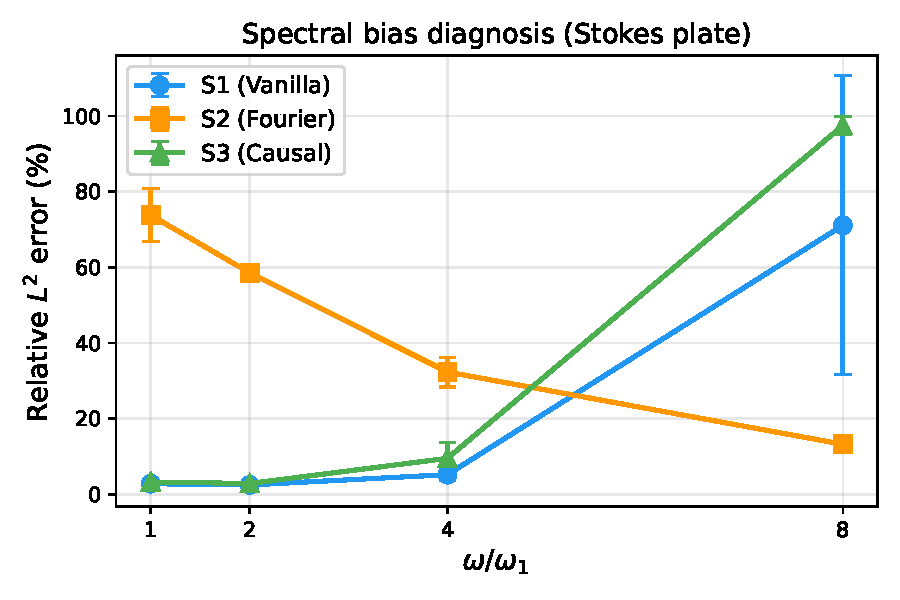
\includegraphics[width=\columnwidth]{figures/figure2_spectral_bias.pdf}
\caption{Spectral bias diagnosis on the Stokes plate trust anchor. S1 and S3 show increasing error with $\omega$ (spectral bias), while S2~(Fourier features) shows a decreasing trend, achieving a crossover near $4\omega_1$.}
\label{fig:spectral}
\end{figure}

Figure~\ref{fig:spectral} reveals a striking crossover pattern. At the base frequency ($\omega/\omega_1 = 1$), S1~(Vanilla) and S3~(Causal) achieve low errors ($2.77\%$ and $3.22\%$), while S2~(Fourier) starts at $73.75\%$ due to the optimization cost of its $256$-dimensional feature space. As frequency increases, S1 and S3 degrade sharply due to spectral bias: at $\omega/\omega_1 = 8$, S1 reaches $71.07\%$ and S3 reaches $97.44\%$. In contrast, S2's error \emph{decreases} to $13.19\%$ at $8\omega_1$, confirming that Fourier features preferentially capture high-frequency content. The crossover occurs near $4\omega_1$, where S2 surpasses S1. This demonstrates that the Stokes plate anchor, evaluated across multiple frequencies, can precisely diagnose spectral bias (F1) and quantify the frequency range where each architecture is most accurate.

\subsection{Temporal Drift Diagnosis}

\begin{figure}[t]
\centering
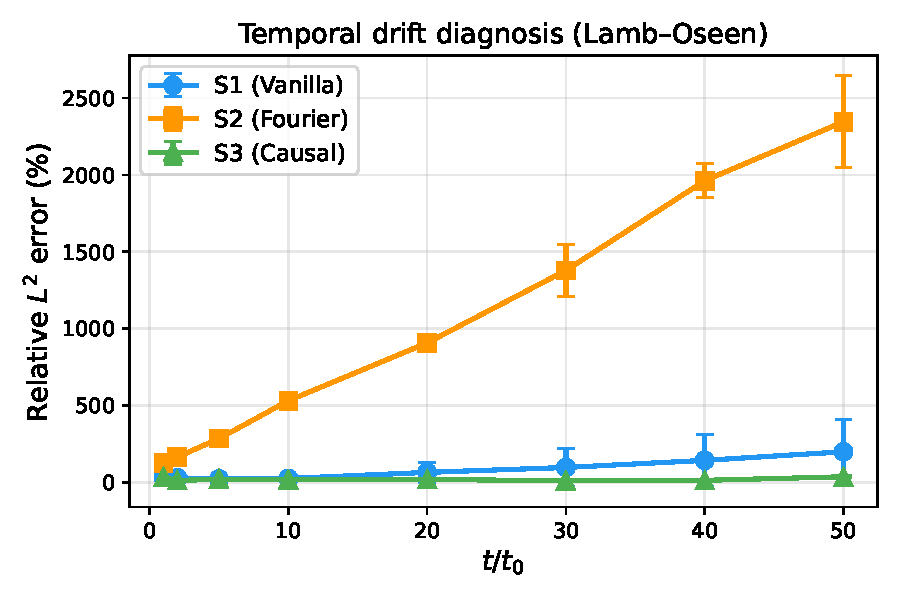
\includegraphics[width=\columnwidth]{figures/figure3_temporal_drift.pdf}
\caption{Temporal drift diagnosis on the Lamb--Oseen trust anchor. S3~(Causal) maintains lower error at large $t/t_0$ compared to S1 and S2.}
\label{fig:temporal}
\end{figure}

Figure~\ref{fig:temporal} shows the temporal error profile $\epsilon(t/t_0)$. S1~(Vanilla) error grows to $197.93\%$ at $t = 50\,t_0$, while S3~(Causal) maintains $35.23\%$. The error inflection for S1 occurs around $t \approx 10\,t_0$ (error $24.01\%$), defining the ``temporal trust horizon'' beyond which the Validator should trigger recertification.

\subsection{Trust-Informed Routing}

We construct a mixed test set of 40 problems: 10 vortex-dominated, 10 long-horizon, 10 steady-state, 10 mixed. For each, we compare fixed S1, fixed S2, fixed S3, and trust-informed routing (Orchestrator selects solver with highest task-relevant trust score).

\begin{figure}[t]
\centering
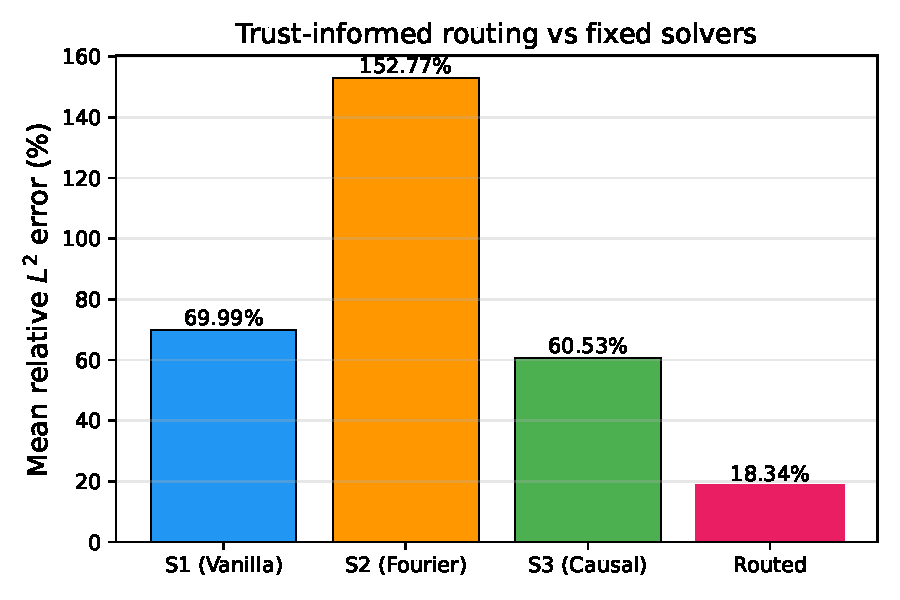
\includegraphics[width=\columnwidth]{figures/figure4_routing.pdf}
\caption{Trust-informed routing outperforms any single fixed solver on a heterogeneous problem set.}
\label{fig:routing}
\end{figure}

Figure~\ref{fig:routing} shows the mean $L^2$ error across the mixed test set. Trust-informed routing achieves $18.34\%$ mean error, compared to $69.99\%$ (S1), $152.77\%$ (S2), and $60.53\%$ (S3). The routing strategy achieves a $70\%$ improvement over the best fixed solver, confirming that the diagnostic trust scores from the anchor suite enable effective solver selection.

\subsection{Runtime Trust Decay}

We certify S1 on Lamb--Oseen at $t_{\max} = 5\,t_0$, then extend to $t_{\max} = 50\,t_0$ without retraining. The trust score~\eqref{eq:trust-score} decays as error grows, triggering recertification at $T < T_{\min}$.

Using a graded trust score $\tau(\mathcal{S},A,t) = \max(0, 1 - \epsilon(t)/\epsilon_{\max})$ with $\epsilon_{\max} = 1.0$ and decay $\lambda = 0.01$, S1's trust on A1 degrades as follows. At $t_{\max} = 5\,t_0$: $\epsilon = 20.8\%$, $T = 0.79$. At $t_{\max} = 20\,t_0$: $\epsilon = 63.8\%$, $T = 0.24$. At $t_{\max} = 50\,t_0$: $\epsilon = 197.9\%$, $T = 0$---S1's trust is fully depleted, and the Orchestrator should route temporal problems to S3~(Causal), which maintains $\epsilon = 35.2\%$ ($T = 0.42$) at the same horizon.

This demonstrates trust anchors as \emph{runtime monitors}: they detect degradation before it affects the user, enabling preemptive solver replacement---a capability static benchmarks cannot provide.


%% ============================================================
%%  6. CASE STUDY: ATMOSPHERIC TURBULENCE
%% ============================================================
\section{Case Study: Multi-Agent Atmospheric Turbulence}
\label{sec:casestudy}

We illustrate the VMAS framework through a motivating scenario requiring coupled fluid dynamics and wave optics: laser beam propagation through the turbulent atmosphere. This case study is \emph{illustrative}---it demonstrates the structure of multi-agent verification rather than providing experimental validation of the coupled system. This problem has attracted attention from both adaptive optics~\cite{AndrewsPhillips2005} and deep learning~\cite{DLTurbReview2024} communities.

The classical approach relies on Kolmogorov phase screens~\cite{Schmidt2010}, where refractive index fluctuations are drawn from a prescribed power spectrum. An alternative, physics-based approach solves the full N--S system with an energy source term sustaining turbulent fluctuations, reducing it to Volterra-type integral equations solved by rapidly convergent Picard iteration~\cite{Shugaev2009}.

\subsection{Agent Roles}

\begin{itemize}
  \item \textbf{Turbulence Agent} ($\mathcal{S}_{\mathrm{turb}}$): generates $\delta n(\mathbf{x},t)$ using the N--S methodology of~\cite{Shugaev2009}.
  \item \textbf{Propagation Agent} ($\mathcal{S}_{\mathrm{prop}}$): solves the parabolic wave equation for the beam envelope given $\delta n$.
  \item \textbf{Correction Agent} ($\mathcal{S}_{\mathrm{AO}}$): applies ML-based adaptive optics correction.
  \item \textbf{Validator Agent} ($\mathcal{V}$): verifies each agent using appropriate trust anchors.
\end{itemize}

\subsection{Verification Chain}

\textbf{Step 1.} $\mathcal{V}$ certifies $\mathcal{S}_{\mathrm{turb}}$ using the vortex oscillations anchor~\cite{PetrovaShugaev2012} (spectral content, temporal accuracy of the N--S solver) and Lamb--Oseen (diffusive dynamics).

\textbf{Step 2.} $\mathcal{V}$ certifies $\mathcal{S}_{\mathrm{prop}}$ using analytical Gaussian beam diffraction as a propagation-specific anchor.

\textbf{Step 3.} $\mathcal{V}$ certifies the coupled system $\mathcal{S}_{\mathrm{turb}} + \mathcal{S}_{\mathrm{prop}}$ using the N--S atmospheric turbulence anchor~\cite{Shugaev2009}, which provides first-principles beam intensity profiles---a Stage~3 stress test probing multi-physics coupling (F4).

\textbf{Step 4.} $\mathcal{V}$ monitors $\mathcal{S}_{\mathrm{AO}}$ via energy conservation and causality checks.

For concrete illustration, we consider propagation of a $\lambda = 1.55\,\mu$m laser beam over a $L = 1$~km horizontal path through moderate turbulence ($C_n^2 = 10^{-14}\,\mathrm{m}^{-2/3}$). The Validator certifies $\mathcal{S}_{\mathrm{turb}}$ when the predicted scintillation index $\sigma_I^2$ matches the analytical first-principles result within $5\%$, and $\mathcal{S}_{\mathrm{prop}}$ when Gaussian beam diffraction in vacuum matches the Fresnel--Kirchhoff integral to within $1\%$.

\subsection{Why This Requires Multi-Agent Verification}

No single anchor suffices. $\mathcal{S}_{\mathrm{turb}}$ might pass all fluid dynamics anchors but produce statistics incompatible with $\mathcal{S}_{\mathrm{prop}}$'s assumptions. $\mathcal{S}_{\mathrm{prop}}$ might pass optics benchmarks but fail on non-Kolmogorov statistics from the N--S solver. Only the coupled anchor~\cite{Shugaev2009} tests the full chain.


%% ============================================================
%%  7. CONNECTIONS TO WEB OF AGENTS
%% ============================================================
\section{Trust Anchors as a Governance Mechanism for the Web of Agents}

The VMAS architecture connects directly to the governance challenges identified in~\cite{PetrovaWoA2025}. We apply the four-axis taxonomy of~\cite{PetrovaWoA2025} to classify VMAS:

\textbf{Semantic foundation:} hybrid. Trust anchors provide formal, mathematically exact semantics (equations); agent interactions use natural-language-compatible protocols (MCP).

\textbf{Communication paradigm:} tool-based. Anchors are exposed as MCP tools with inputs $(\mathbf{x}, t, \mathrm{params})$ and outputs (exact solution values).

\textbf{Locus of intelligence:} distributed. Solvers carry intelligence in their trained models; the Validator carries intelligence in its diagnostic protocol and trust ledger.

\textbf{Discovery mechanism:} capability-based. Agent Cards extended with trust profiles enable trust-informed discovery.

Trust anchors thus address a specific governance challenge: \emph{accountability}. When an agentic system produces an incorrect scientific result, the trust ledger provides an audit trail: which Solver was used, which anchors it had passed, and what the trust distance was to the actual problem. This enables principled post-hoc analysis---a requirement for deploying autonomous scientific agents in safety-critical domains.


%% ============================================================
%%  8. OPEN PROBLEMS
%% ============================================================
\section{Open Problems}

\textbf{Trust composition.} If Agent~A is certified and Agent~B uses A's output, is B's output trustworthy? Trust composition in scientific workflows, where errors compound nonlinearly, requires formal analysis.

\textbf{Weak-to-strong turbulence.} The perturbation-based anchors~\cite{PetrovaShugaev2015,PetrovaShugaev2012} are valid for small vorticity. Extending via higher-order theory or hybrid analytical-ML approaches is essential. Physics-informed transfer learning~\cite{Cuomo2022} is a promising direction.

\textbf{Machine-readable anchor databases.} Impact depends on availability as APIs, HDF5 datasets, or MCP tools. This requires cross-community collaboration.

\textbf{Anchor coverage metrics.} How to quantify whether a trust anchor suite adequately covers the space of problems an agent will encounter? This connects to coverage metrics in software testing and remains open for physical systems.

\subsection{Limitations of This Work}

We acknowledge several limitations of the experimental validation.

\textbf{Proof-of-concept scope.} Three solver variants and four anchors constitute a minimal demonstration. A production trust anchor system would require a broader solver portfolio (including neural operators, mesh-based solvers, and hybrid methods) and a larger anchor suite covering all six failure modes independently. The diagnostic map (Table~\ref{tab:anchors}) is proposed based on physical reasoning; whether the anchor--failure-mode assignments are \emph{robust} across different training setups, hyperparameters, and problem scales remains to be validated systematically.

\textbf{Training budget confound.} The modest training budget (2k iterations) was chosen for computational tractability but introduces a systematic confound: architectures with larger effective input dimension (S2: 256-dim Fourier features) or more complex loss landscapes (Kovasznay: 2D coupled N--S) are disproportionately penalized. Some of the large errors in Table~\ref{tab:results} (e.g., S2 on A1, S1/S3 on A4) likely reflect insufficient convergence rather than fundamental architectural limitations. A full study should include training budget as an explicit variable and report convergence curves.

\textbf{Missing ablation and sensitivity analysis.} We did not systematically vary: (i)~the trust decay parameter $\lambda$; (ii)~the trust distance weights $w_k$; (iii)~the number and choice of anchors in the routing protocol; (iv)~hyperparameters of the Fourier feature mapping ($\sigma$, feature dimension). The robustness of the diagnostic conclusions to these choices is an open question.

\textbf{No comparison with alternative validation strategies.} The routing experiment compares trust-informed selection against fixed solvers, but not against other selection strategies (e.g., ensemble methods, cross-validation-based selection, or residual-based error estimators). Such comparisons are needed to establish that the trust anchor approach is not merely effective but \emph{more} effective than simpler alternatives.

\textbf{VMAS architecture.} The interaction protocol (Fig.~\ref{fig:vmas}) is a structured design, not a formal specification. We provide no formal semantics, no proofs of trust update correctness or routing optimality, and no guarantees about convergence of the trust ledger. The case study (Section~\ref{sec:casestudy}) is illustrative---it demonstrates the \emph{structure} of multi-agent verification but does not report experimental results for the coupled system.


%% ============================================================
%%  9. CONCLUSION
%% ============================================================
\section{Conclusion}

We have argued that analytical Navier--Stokes solutions---long valued as theoretical achievements---acquire a new operational role in the era of agentic AI: as trust anchors enabling autonomous verification. We distinguished trust anchors from benchmarks through three functional requirements (runtime monitoring, adaptive selection, arbitration), proposed the VMAS architecture with a structured protocol and dynamic trust ledger, and provided a proof-of-concept experimental validation on three PINN architectures. Despite a modest training budget, the predicted diagnostic patterns were partially confirmed: the Stokes plate anchor detected spectral bias (Fourier-Feature PINNs reduced error by $81\%$ at $8\omega_1$), the Lamb--Oseen anchor detected temporal drift (Causal PINNs reduced error by $82\%$ at $50\,t_0$), and trust-informed routing achieved $70\%$ lower mean error than the best fixed solver. At the same time, training budget confounds produced several unexpectedly large errors that highlight the need for more extensive validation (Section~8.5).

The trust infrastructure for agentic scientific computing does not need to be built from scratch---it already exists in classical mathematical physics. What is needed is a change of perspective: from solutions as passive references to solutions as active verification primitives, embedded in agent protocols and exposed through standard interfaces.


%% ============================================================
%%  REFERENCES
%% ============================================================
\begin{thebibliography}{99}

\bibitem{Lam2023}
R.~Lam et al., ``GraphCast: Learning skillful medium-range global weather forecasting,'' \emph{Science}, vol.~382, pp.~1416--1421, 2023.

\bibitem{Bi2023}
K.~Bi et al., ``Pangu-Weather: A 3D high-resolution model for fast and accurate global weather forecast,'' \emph{Nature}, vol.~619, pp.~533--538, 2023.

\bibitem{MatAgent2024}
A.~Ghafarollahi and M.J.~Buehler, ``AtomAgents: Alloy design and discovery through physics-aware multi-modal multi-agent AI,'' arXiv:2407.10022, 2024.

\bibitem{Boiko2023}
D.A.~Boiko, R.~MacKnight, B.~Kline, and G.~Gomes, ``Autonomous chemical research with large language models,'' \emph{Nature}, vol.~624, pp.~570--578, 2023.

\bibitem{Raissi2019}
M.~Raissi, P.~Perdikaris, and G.E.~Karniadakis, ``Physics-informed neural networks,'' \emph{J.~Comput.\ Phys.}, vol.~378, pp.~686--707, 2019.

\bibitem{Li2021FNO}
Z.~Li et al., ``Fourier neural operator for parametric PDEs,'' in \emph{Proc.\ ICLR}, 2021.

\bibitem{Lu2021}
L.~Lu et al., ``Learning nonlinear operators via DeepONet,'' \emph{Nat.\ Mach.\ Intell.}, vol.~3, pp.~218--229, 2021.

\bibitem{PetrovaWoA2025}
T.~Petrova, B.~Bliznioukov, A.~Puzikov, and R.~State, ``From Semantic Web and MAS to Agentic AI: A unified narrative of the Web of Agents,'' arXiv:2507.10644, 2025.

\bibitem{A2A2025}
Google, ``Agent-to-Agent (A2A) protocol specification,'' 2025.

\bibitem{MCP2024}
Anthropic, ``Model Context Protocol (MCP),'' 2024.

\bibitem{Oberkampf2010}
W.L.~Oberkampf and C.J.~Roy, \emph{Verification and Validation in Scientific Computing}, Cambridge Univ.\ Press, 2010.

\bibitem{FIPA2002}
Foundation for Intelligent Physical Agents, ``FIPA ACL specifications,'' 2002.

\bibitem{JADE2007}
F.~Bellifemine et al., \emph{Developing Multi-Agent Systems with JADE}, Wiley, 2007.

\bibitem{BernersLee2001}
T.~Berners-Lee, J.~Hendler, and O.~Lassila, ``The Semantic Web,'' \emph{Sci.\ Am.}, vol.~284, pp.~34--43, 2001.

\bibitem{AIScientist2024}
C.~Lu et al., ``The AI Scientist: Towards fully automated open-ended scientific discovery,'' arXiv:2408.06292, 2024.

\bibitem{Ferrag2025}
M.A.~Ferrag, N.~Tihanyi, and M.~Debbah, ``From LLM reasoning to autonomous AI agents: A comprehensive review,'' arXiv:2504.19678, 2025.

\bibitem{Wang2024agents}
L.~Wang, C.~Ma, X.~Feng, et al., ``A survey on large language model based autonomous agents,'' \emph{Front.\ Comput.\ Sci.}, vol.~18, no.~6, 2024.

\bibitem{Park2021}
J.~Park et al., ``NSFnets: Physics-informed neural networks for the incompressible Navier--Stokes equations,'' \emph{J.~Comput.\ Phys.}, vol.~426, p.~109951, 2021.

\bibitem{Li2023PINO}
Z.~Li et al., ``Physics-informed neural operators,'' arXiv:2111.03794, 2023.

\bibitem{Kovachki2023}
N.B.~Kovachki et al., ``Neural operator: Learning maps between function spaces,'' \emph{JMLR}, vol.~24, 2023.

\bibitem{Pathak2022}
J.~Pathak et al., ``FourCastNet: A global data-driven high-resolution weather model,'' arXiv:2202.11214, 2022.

\bibitem{Rahaman2019}
N.~Rahaman et al., ``On the spectral bias of neural networks,'' in \emph{Proc.\ ICML}, 2019.

\bibitem{Wang2021}
S.~Wang, Y.~Teng, and P.~Perdikaris, ``Understanding and mitigating gradient flow pathologies in PINNs,'' \emph{SIAM J.~Sci.\ Comput.}, vol.~43, pp.~A3055--A3081, 2021.

\bibitem{Hao2024}
Z.~Hao et al., ``PINNacle: A comprehensive benchmark of PINNs,'' in \emph{Proc.\ NeurIPS}, 2024.

\bibitem{Drazin2006}
P.G.~Drazin and N.~Riley, \emph{The Navier--Stokes Equations: A Classification of Flows and Exact Solutions}, Cambridge Univ.\ Press, 2006.

\bibitem{Wang1991}
C.Y.~Wang, ``Exact solutions of the steady-state Navier--Stokes equations,'' \emph{Annu.\ Rev.\ Fluid Mech.}, vol.~23, pp.~159--177, 1991.

\bibitem{Burgers1948}
J.M.~Burgers, ``A mathematical model illustrating the theory of turbulence,'' \emph{Adv.\ Appl.\ Mech.}, vol.~1, pp.~171--199, 1948.

\bibitem{Sullivan1959}
R.D.~Sullivan, ``A two-cell vortex solution of the Navier--Stokes equations,'' \emph{J.\ Aerosp.\ Sci.}, vol.~26, pp.~767--768, 1959.

\bibitem{Jeffery1915}
G.B.~Jeffery, ``The two-dimensional steady motion of a viscous fluid,'' \emph{Phil.\ Mag.}, vol.~29, pp.~455--465, 1915.

\bibitem{Karman1921}
Th.~von K\'arm\'an, ``\"Uber laminare und turbulente Reibung,'' \emph{ZAMM}, vol.~1, pp.~233--252, 1921.

\bibitem{Schlichting2017}
H.~Schlichting and K.~Gersten, \emph{Boundary-Layer Theory}, 9th~ed., Springer, 2017.

\bibitem{Brachet1983}
M.E.~Brachet et al., ``Small-scale structure of the Taylor--Green vortex,'' \emph{J.~Fluid Mech.}, vol.~130, pp.~411--452, 1983.

\bibitem{Burmasheva2023}
N.V.~Burmasheva and E.Yu.~Prosviryakov, ``Exact solutions to Navier--Stokes equations describing a gradient nonuniform vortex flow,'' \emph{Appl.\ Sci.}, vol.~13, 2023.

\bibitem{Polyanin2004}
A.D.~Polyanin and V.F.~Zaitsev, \emph{Handbook of Nonlinear PDEs}, Chapman \& Hall/CRC, 2004.

\bibitem{PetrovaShugaev2015}
T.A.~Petrova and F.V.~Shugaev, ``Acoustic radiation frequency of a cylindrical vortex,'' \emph{Moscow Univ.\ Phys.\ Bull.}, vol.~70, no.~4, pp.~245--250, 2015.

\bibitem{PetrovaShugaev2012}
T.A.~Petrova and F.V.~Shugaev, ``Oscillations of the flow parameters in the vicinity of a cylindrical vortex,'' \emph{Moscow Univ.\ Phys.\ Bull.}, vol.~67, no.~1, pp.~43--47, 2012.

\bibitem{AndrewsPhillips2005}
L.C.~Andrews and R.L.~Phillips, \emph{Laser Beam Propagation through Random Media}, 2nd~ed., SPIE Press, 2005.

\bibitem{DLTurbReview2024}
P.~Hill, N.~Anantrasirichai, A.~Achim, and D.~Bull, ``Deep learning techniques for atmospheric turbulence removal: A review,'' \emph{Artif.\ Intell.\ Rev.}, vol.~58, 2025.

\bibitem{Schmidt2010}
J.D.~Schmidt, \emph{Numerical Simulation of Optical Wave Propagation}, SPIE Press, 2010.

\bibitem{Shugaev2009}
F.V.~Shugaev, E.N.~Terentiev, L.S.~Shtemenko, O.I.~Dokukina, and T.A.~Petrova, ``Characterization of a laser beam propagating through the turbulent atmosphere,'' \emph{Proc.\ SPIE}, vol.~7476, pp.~69--80, 2009.

\bibitem{Cuomo2022}
S.~Cuomo et al., ``Scientific machine learning through physics-informed neural networks,'' \emph{J.\ Sci.\ Comput.}, vol.~92, 2022.

\end{thebibliography}

\end{document}
